\subsection{投票と技術}
今まで見てきた投票方式にも例えば承認投票や勝ち抜き方式のように票の集計が難しいものがあります.勝ち抜き方式では選択肢の数(n個) $\times$ 個人の数(m個)のデータを扱う必要があります.この場合各投票用紙のn個のデータをm回集計したあと順番に並べるので,$O(mn)$の時間計算量です.多項式時間で集計できないような方式なら別ですが,この場合,電子投票ならば集計が一瞬で終わります.そうすると,今まで選挙にまとわりついていた様々な制約が消え,選挙制度や政治制度の変革が起こりえます.

また,架空世界創作という観点に立てば,情報通信技術でできることは魔法でもできるかもしれません.魔法世界での社会的決定で我々が行っているような単記投票ばかりが用いられていると考えるのはむしろ不自然なのかもしれません.具体的に魔法がどのようなものかについての考察はしませんが,魔法のある架空世界の創作者は,その世界の魔法が情報や通信に応用できるならどのように投票にも応用できるのかを考えてみるといいかもしれません.

一般にどのような組織も自分で自分を規制するルールを制定することには消極的なので,一票の格差是正などの問題を国会の議論だけに任せてもその場しのぎの対策だけで済まされてしまうことでしょう.選挙制度を決めるのが人間である限りは選挙制度改革はなかなか進みません.情報技術の進歩した社会においては選挙制度の決定も機械的に処理されるものだと考えるべきでしょう.

\subsubsection*{オンライン投票と集計作業の自動化}
有権者がパソコンや携帯端末を用いて投票することについて考えてみましょう.

最初に問題になるのはすべての有権者がパソコンや携帯端末を保有しているのかという問題です.当然ですが,有権者のほぼ全員が情報通信機器にアクセスできなければ電子投票は不可能です.現在の日本では携帯端末機器の世帯保有率は9割を超えていています\footnote{情報通信白書 平成29年度版 第1部 第1章 第1節 図1-1-1-1}.SFなどで出てくる世界観や科学技術観はその当時の水準に影響されるように思いますし\footnote{特に根拠はないですが.},現在含め今後,架空世界創作の中でほぼすべての有権者が携帯端末を保有し操作できる架空世界が多数現れることは想像に難くないでしょう\footnote{というか,すでにそういう世界観の作品は多数あるっぽいです.}\footnote{そのような世界では,携帯端末を保有していないことが経済的格差の象徴とされるかもしれません.格差のあり方によっては携帯機器不保持で個人認証ができないために投票できないということも考えられます.まあ,創作という観点から見るとそのような層を登場させないことで格差を隠すこともできますが,投票という観点から見ると考慮すべき事案かもしれません.}.そのような世界では,電子投票・オンライン投票の利点が大きそうです.利点について考えてみましょう.

まず,有権者が自分の携帯端末から投票するならば,自治体は多数の投票所を設置する必要もありませんし,開票作業に多額の人件費をかける必要もありません.現在,日本では一回の国政選挙で全国約5万箇所の投票所が必要で\footnote{http://www.soumu.go.jp/senkyo/48sansokuhou/index.html},選挙のたびに600億円以上もの費用がかかります\footnote{http://www.soumu.go.jp/main\_content/000506000.pdf}.さらに有権者が投票所に出向く必要もなくなります.投票所に出向く必要があると,投票日に雨が降ったりすると投票率が落ちたりするので,どこでも投票できるのは利便性だけでなく,投票率向上の効果も期待できそうです.携帯端末からの投票なので,全国どこからでも,国外からでも容易に投票が可能です.投票期間を一日に限定せず,長めに取ることもできます\footnote{この場合,すでに投票した個人が期日前に死亡すると投票は無効になるんでしょうか?}.また,投票の内容を期日中ならなんどでも変更するということも可能です.これは,他人による意志の強要などの回避にもつながります.便利で気軽に投票できるシステムであれば,社会的決定への参加がより身近になり,投票率向上などの様々な利点があると考えられます.他にも,無効票の投票がシステム的に不可能など,無数に利点が挙げられるのではないでしょうか.

投票においては不正投票の防止のために個人認証が必要になります.指紋や声紋などでの認識など様々な方法が考えられます.情報通信機器による個人認証はなりすましが容易なのではないかとも考えられますが,日本の国政選挙で行われているハガキと立会人の目視\footnote{性別や年齢などを確認するらしいです.}による本人確認も,誰が住んでるかよくわからない都会でなら同様になりすましが容易でしょうし,電子投票の方がなりすましが困難なような認証方法も考えられるでしょうから,個々の架空世界の技術でなんとかなると思うので,なんとかしてください.

集計もすべて自動化が可能となり,人選費の削減や開票作業が正確で高速なものになります.必要な人手はシステムの起動や開票結果の公表程度です.コスト全体ではシステムの運用・保守のためのコストが最も大きな割合を占めるでしょうが,人力でやるのに比べると僅かなものです.選挙期間中に自治体の業務が増えることもなく,職員の休日出勤も不要になります.

\subsubsection*{区割りの最適化による格差是正}
多数の議員を選出する時,共同体全体を地域や部族などに分ける選挙区を導入することがあります.この時問題となるのが,一票の格差や特定の候補に有利になるような区割り\footnote{いわゆるゲリマンダーです.}がされたりすることです.人間が区割りをする以上は様々な思惑が介入するでしょうし,区割りも自動的に決めるべきという考え方もできるかもしれません.

一票の格差を是正するためには,すべての選挙区の有権者数を一定の範囲内に収める必要があります\footnote{なるべく,$\frac{全有権者数}{議員定数}\times 選出議員数に近づくようにします.$}.この場合,地域全体を地域特性等を考慮して数百人・数千人規模ごとに分割し,適切に併合していくという組み合わせ最適化問題とすればよいでしょう\footnote{人口統計調査や人種分布・言語分布などをもとに少数者に不利にならないようにしながら,なるべく区割りが歪な形にならないようにするとよいかもしれません.}.このような区割りを選挙前に自動的に行い,選挙運動が始まる前に公表することになります.

選挙制度改革でこのように区割りの最適化を毎回行うというのは,多くの議員にとって好ましいことではないでしょう.なぜならば,議員にはその選挙区の有権者との密接な人間関係があるかもしれないからです\footnote{いわゆる地盤です.}.機械的な区割りの決定によって既存の選挙区と大きく区画が変わった場合,今まで当選確実だった候補が再選を果たせなくなることも考えられます.そのことも考慮すれば,選挙の後に次の選挙で用いる区割りを予め決めておくという方法も有効かもしれません.ただ,民主的社会であるならば,個人の平等性,すなわち一票の格差が少ない状態であることは優先されるべきですし,個々の議員の地盤に配慮するべきではないのかもしれません.いくら有能な人材であっても,多数の支持を得られなければ選出されないのは仕方がないことではあります.

\subsubsection*{シュルツ方式}
単記投票の開票・集計作業の時間計算量は選択肢mつ,個人n人とすれば,$O(n)$です.ボルダ得点でも$O(mn)$です.一方,多数決決定法だと$O(m^2 n)$です\footnote{選択肢のペア$_mC_2 = \frac{m(m-1)}{2}$個に対する個人的選好をn人分集計するので.}.$O(n^2)$のような方式はあまりないと思いますが,もしそのような方式があれば,$n = 1,000$ともなれば,開票作業は人力では到底一晩では終わりません.しかし,電子投票で集まったデータを集計するなら,この程度はすぐ終わります.

シュルツ方式という方式があります.多数決決定法のように個人の選好をすべて反映させますが,社会的選好が非循環性を満たす方式です.多数決決定法では2選択肢のどちらを選好する個人が多いかで社会的選好を決めます.しかし,それだと社会的に循環が起こりますが,シュルツ方式では様々な選択肢間の選好まで見て循環しないように社会的選好を決めて循環を回避しています.

シュルツ方式では,2選択肢間の道と,その道の強さというものを考えて社会的決定をします.

\begin{dfn}
    $d(x,y)$は$x>y$と選好する個人の数です.    
\end{dfn}
\begin{dfn}[道]
    選択肢$x_0$から$x_{n-1}$への道とは,$\forall i (d(x_i,x,{i+1}) > d(x_{i+1},x_i))$を満たすような異なるn個の選択肢$x_0,x_1,\dots,x_{n-1}$の列のことです.
\end{dfn}
ただし,始点と終点が同じであるような道について考えるときだけは,始点と終点の重複を許すことにします.
\begin{dfn}[道の強さ]
    選択肢$x_0$から$x_{n-1}$への道において道の強さとは,\\$d(x_0,x_1),d(x_1,x_2),\dots,d(x_{n-2},x_{n-1})$の最小値のことです.そのような道が存在しない場合は強さを0とします.
\end{dfn}
\begin{dfn}
    選択肢$x$から$y$への道の強さの最大値を$p(x,y)$とします.
\end{dfn}
\begin{dfn}[シュルツ方式]
    シュルツ方式とは,社会的選好を
    \begin{equation*}
        x \succeq y \leftrightarrow p(x,y) \geq p(y,x)
    \end{equation*}
    とする決定方式のことです.
\end{dfn}

個人的選好を図35のようにします.
\begin{figure}[!h]
    \centering
    \begin{tabular}[!h]{|c|c|c|c|c|c|} \hline
          & 8人 & 2人 & 4人 & 4人 & 3人 \\ \hline
        1 & x   & y   & z   & w   & w   \\ \hline
        2 & z   & x   & w   & y   & z   \\ \hline
        3 & w   & w   & y   & x   & y   \\ \hline
        4 & y   & z   & x   & z   & x   \\ \hline
    \end{tabular}
    \caption{個人的選好}
\end{figure}
このとき,すべての選択肢のペアに対して図36のようになります.
\begin{figure}[!h]
    \centering
    \begin{tabular}[!h]{|c|c|c|c|c|} \hline
               & d(*,x) & d(*,y) & d(*,z) & d(*,w) \\ \hline
        d(x,*) &        &  8     & 14     & 10     \\ \hline
        d(y,*) & 13     &        &  6     &  2     \\ \hline
        d(z,*) &  7     & 15     &        & 12     \\ \hline
        d(w,*) & 11     & 19     &  9     &        \\ \hline
    \end{tabular}
    \caption{$d(*,*)$}
\end{figure}

2選択肢について,選好する人が少ない選択肢を始点,多い選択肢を終点とする辺による有向グラフを考えれば,道の強さ$p(x,y)$はそのグラフでxからyへの道での途中の辺の強さの最小値となります.
\begin{figure}[!h]
    \centering
    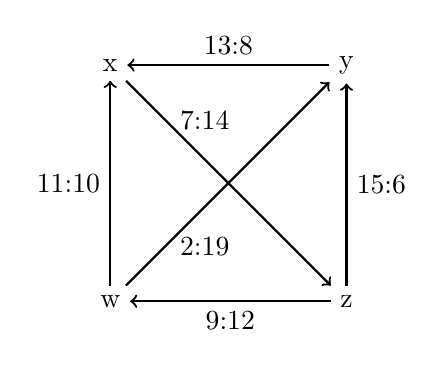
\begin{tikzpicture}
        \node (x) at (0,3) {x};
        \node (y) at (3,3) {y};
        \node (z) at (3,0) {z};
        \node (w) at (0,0) {w};
        \draw[thick, <-] (x) -- node[above]{13:8} (y);
        \draw[thick, ->] (x) -- (z);
        \draw[thick, <-] (x) -- node[left]{11:10} (w);
        \draw[thick, <-] (y) -- node[right]{15:6} (z);
        \draw[thick, <-] (y) -- (w);
        \draw[thick, ->] (z) -- node[below]{9:12} (w);
        \node (1) at (1.2,2.3) {7:14};
        \node (2) at (1.2,0.7) {2:19};
    \end{tikzpicture}
    \caption{グラフ}
\end{figure}
グラフは図37のようになります.図37より,図38のようになります.
\begin{figure}[!h]
    \centering
    \begin{tabular}[!h]{|c|c|c|c|c|} \hline
               & p(*,x) & p(*,y) & p(*,z) & p(*,w) \\ \hline
        p(x,*) &        & 14     & 14     & 12     \\ \hline
        p(y,*) & 13     &        & 13     & 12     \\ \hline
        p(z,*) & 13     & 15     &        & 12     \\ \hline
        p(w,*) & 13     & 19     & 13     &        \\ \hline
    \end{tabular}
    \caption{$p(*,*)$}
\end{figure}
図38より,$w \succ x \succ z \succ y$です.

ところで,図35$\sim$図38の例では社会的選好に推移性と非循環性が成立していることが確認できますが,どのような場合でも推移性や非循環性が成立しているのでしょうか?

推移性は満たしていません.例えば,$x > y > z, x > z > y, y > x > z, z > y > x$とする個人が1人ずついる場合,$p(x,y) = p(y,x) = p(y,z) = p(z,y) = p(z,x) = 2$ですが,$p(x,z) = 3$となり,$x \simeq y \land y \simeq z$なのに,$x \succ z$となり,推移性は満たしません.

非循環性は常に成立することが証明できます.そのことを証明する前に少しシュルツ方式の性質について述べることにします.

\begin{lem}
    シュルツ方式では,任意の異なる3選択肢x,y,zに対して,
    \begin{equation*}
        min\{p(x,y),p(y,z)\} \leq p(x,z)
    \end{equation*}
    が成り立ちます.また,
    \begin{equation*}
        p(x,y) \leq p(x,z) \lor p(y,z) \leq p(x,z)
    \end{equation*}
    が成り立ちます.
\end{lem}
\begin{proof}
xからzへ至るすべての道の強さの最大値が$p(x,z)$です.ここで,xからyへ至る強さ$p(x,y)$の道とyからzへ至る強さ$p(y,z)$の道がともに存在するならば,それらを合わせた道の強さは$min\{p(x,y),p(y,z)\}$となります.xからzへ至る道の強さは$p(x,z)$以下なので,$min\{p(x,y),p(y,z)\} \leq p(x,z)$となります.xからyへの道かyからzへの道のどちらかまたは両方が存在しない場合は,$min\{p(x,y),p(y,z)\} = 0$なので,条件は常に成立します.

$min\{p(x,y),p(y,z)\} \leq p(x,z)$から,それと同値な命題$p(x,y) \leq p(x,z) \lor p(y,z) \leq p(x,z)$が成り立つこともわかります.
\end{proof}

次に述べるのはシュルツ方式の説明ではないですが,シュルツ方式の性質を証明するのに使うものです.
\begin{dfn}[擬推移性]
    任意の二項関係$R$は,任意の3つの選択肢の組$x,y,z$に対して,$xPy \land yPz \to xPz$を満たすとき擬推移性を持つと言います.ただし,$P$は,$xPy \leftrightarrow xRy \land \sim yRx$です.
\end{dfn}
$R$が$\geq,\succeq$,$P$が$>,\succ$に対応します.
\begin{lem}
    推移性を持つ二項関係は擬推移性も持ちます.また,擬推移性を持つ二項関係は非循環性も持ちます.
\end{lem}
\begin{proof}
(推移性$\to$擬推移性)二項関係$R$が推移性を持つとします.この時,$xPy \land yPz \to xPz$を示せば良いので,前件$xPy \land yPz$を仮定します.推移性より,$xPy \land yPz \to xRy \land yRz \to xRz$.$zRx$を仮定すると,推移性より$zRx \land xRy \to zRy$.しかし,$yPz$より矛盾.よって,背理法より$\sim xRz$です.よって$xPz$となり,$R$は擬推移性も満たします.

(擬推移性$\to$非循環性)二項関係$R$が擬推移性を持つとします.この時$n$個の選択肢$x_1,\dots,x_n$に対して,数学的帰納法より$x_1 P x_2 P \dots P x_n \to x_1 P x_n$です.よって,$x_1 P x_2 P \dots P x_n \to x_1 R x_n$なので,非循環性も満たします.
\end{proof}


\begin{thm}
    シュルツ方式は個人的選好の自由を満たす社会的決定関数です.
\end{thm}

\begin{proof}
シュルツ方式で,どのような選択肢の組に対しても,反射性,完全性,非循環性が成り立つことを示せばよいです.

(反射性)任意の選択肢xに対して,$p(x,x) = p(x,x)$なので,当然$x \succeq x$です.

(完全性)任意の異なる2つの選択肢x,yに対して,整数$p(x,y)$と$p(y,x)$が存在し,$p(x,y) < p(y,x)$または$p(x,y) = p(y,x)$または$p(x,y) > p(y,x)$であり,よって,$x \prec y$または$x \simeq y$または$x \succ y$です.

(非循環性)補題6.2より,擬推移性を満たすことが示せれば良いです.$x \succ y \land y \succ z$を仮定します.この時,$p(x,y) > p(y,x)$かつ$p(y,z) > p(z,y)$です.$x \succ z$を示したいので,$p(x,z) > p(z,x)$となれば良いです.

補題6.1より,$p(x,y) \leq p(x,z) \lor p(y,z) \leq p(x,z)$.$p(x,y) \leq p(x,z)$の時について考えます.この時,$p(x,z) \geq p(x,y) > p(y,x)$です.

補題6.1より,$p(y,z) \leq p(y,x) \lor p(z,x) \leq p(y,x)$.$p(z,x) \leq p(y,x)$の時,$p(x,z) > p(y,x) \geq p(z,x)$より,$x \succ z$です.$p(y,z) \leq p(y,x)$の時,$p(y,z) > p(z,y)$より,$p(x,z) \geq p(x,y) > p(z,y)$です.補題6.1より,$p(z,x) \leq p(z,y) \lor p(x,y) \leq p(z,y)$です.$p(x,y) \leq p(z,y)$の時は,$p(x,y) > p(x,y)$で矛盾します.よって,$p(x,y) \not \leq p(z,y)$とわかり,選言三段論法より$p(z,x) \leq p(z,y)$です.よって,$p(x,z) > p(z,x)$で,$x \succ z$です.

$p(y,z) \leq p(x,z)$の時についても図39の手順を追えば同様に示すことができます.よって非循環性も満たします.

\begin{figure}[!h]
    \centering
    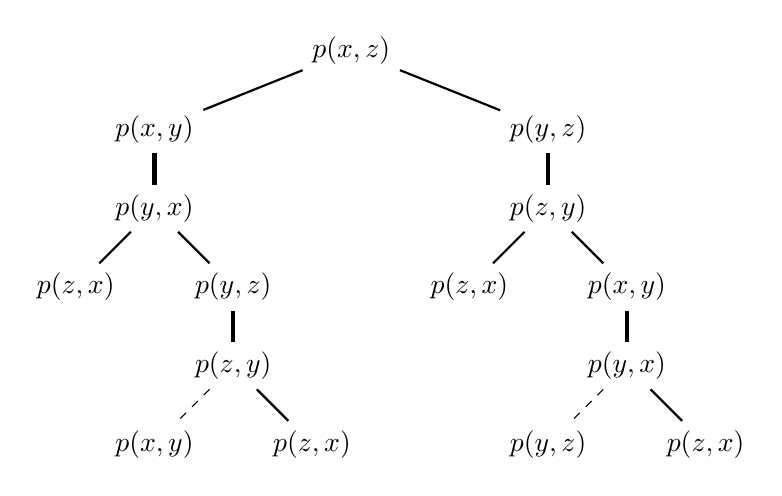
\begin{tikzpicture}
        \node (a) at (3.5,5){$p(x,z)$};
        \node (b) at (1,4) {$p(x,y)$};
        \node (c) at (1,3) {$p(y,x)$};
        \node (d) at (0,2) {$p(z,x)$};
        \node (e) at (2,2) {$p(y,z)$};
        \node (f) at (2,1) {$p(z,y)$};
        \node (g) at (1,0) {$p(x,y)$};
        \node (h) at (3,0) {$p(z,x)$};
        \node (i) at (6,4) {$p(y,z)$};
        \node (j) at (6,3) {$p(z,y)$};
        \node (k) at (5,2) {$p(z,x)$};
        \node (l) at (7,2) {$p(x,y)$};
        \node (m) at (7,1) {$p(y,x)$};
        \node (n) at (6,0) {$p(y,z)$};
        \node (o) at (8,0) {$p(z,x)$};
        \draw[thick]       (a) -- (b);
        \draw[ultra thick] (b) -- (c);
        \draw[thick]       (c) -- (d);
        \draw[thick]       (c) -- (e);
        \draw[ultra thick] (e) -- (f);
        \draw[dashed]      (f) -- (g);
        \draw[thick]       (f) -- (h);
        \draw[thick]       (a) -- (i);
        \draw[ultra thick] (i) -- (j);
        \draw[thick]       (j) -- (k);
        \draw[thick]       (j) -- (l);
        \draw[ultra thick] (l) -- (m);
        \draw[dashed]      (m) -- (n);
        \draw[thick]       (m) -- (o);
    \end{tikzpicture}
    \caption{証明の手順(太線は$>$,細線は$\geq$,点線は矛盾を表します.)}
\end{figure}
\end{proof}
図39から,推移性を満たすだけ,すなわち太線が細線になる時は,点線部分の矛盾が示せないことがわかります.このことからシュルツ方式は社会的には推移性を満たさないことがわかります.逆に,$x \succeq y \succ z \to x \succ z$のような擬順序より弱い条件でも満たすこともわかります.

シュルツ方式は社会的決定関数なわけですから,必ず選択集合が存在します.つまり,投票を行って最良要素を選ぶことができます.これは社会的決定には十分な性質と言えます.

では,シュルツ方式の開票・集計作業の時間計算量はどれだけになるでしょうか.投票データから$d(*,*)$を表にするのに$O(m^2 n)$.$p(*,*)$の表を作るのが少しむずかしいですが,ワーシャル・フロイド法というアルゴリズムを用いれば$O(m^3)$で計算できることが知られています.$p(*,*)$の表から社会的選好を決めるのには$O(m^2)$なので,結局,$O(m^2 n + m^3)$です.

単記投票法が$O(n)$なので,選択肢が数倍程度に増えても単記投票法では手間が大して変わらないのに対して,シュルツ方式は選択肢の増加率のべきに比例する量の開票作業が必要になります.しかし,選択肢の数が急増するとしても高々10倍程度まででしょうし,計算機を用いて開票することを考えればシュルツ方式は集計が不可能な方式ではありません.

シュルツ方式は欠点が少ない方式として知られていて\footnote{無関係選択肢からの独立性は満たしていません.しかし,思うにこれほど複雑な方式だと戦略的投票ができるんだろうかという感じもしますし,あまり大きな欠点ではないのかもしれません.},Debianやウィキメディア財団,Haskellなどで投票方式として使われています.すごそうな方式なのですが,その利点について深く述べることはちょっと大変なのでやめます.詳しいことを知りたい人は参考文献[4]などを参考にしてください.ここで述べたいのは,時間計算量が$O(m^2 n)$のような多数決方法も情報通信機器を利用して電子投票すれば可能だということです.電子投票をする世界では,投票方式についてもこのように多様な選択が可能となります.

\subsection{電子投票な世界はどうなのか}
今まで色々見てきました.現実世界でも電子投票が導入されれば良いのになあという思いもあるわけですが,時期尚早と言われれば,まあそうですね,という感じもします.架空世界ならば電子投票を導入することに積極的な世界もあるでしょうが,そもそも電子投票をする世界では投票だけではなく,メディアによる世論の形成や国民的議論も情報通信機器によってなされるかと思われます.

多数決が民主的とは無関係であること,民主制にとって重要なのは議論と交渉(なのではないか)ということはすでに述べたとおりです.この文書では社会的決定方式の方に重きを置いていますが,それは理論やシステムの話であって,実際に理念として大切なのは意思決定に参加する個々人の意識なのだろうと思います.一体どのようにすれば多様な意見を比較検討するような意思決定ができるのか,個々の架空世界の世界観が大きく反映されるところでしょうし,大雑把にしか述べられませんし,私の稚拙な考えがどこまで役に立つかはわかりませんが,少しだけ考えてみたいと思います.

どれだけ議論を重視するような文化であろうと,誰しもが積極的に議論や交渉に参加できるわけではありません.しかし,そのような人々の意見も民主的な社会的決定には当然反映されるべきです.そこで,投票と議論を段階的に繰り返していくという手法が考えられます.何度も投票・議論を繰り返すことは我々の住む現代においても時間と費用がかかる非常に困難なことですが,情報通信技術が高度に発達した世界では,小規模な投票行為や議論は日常的に行われていることなのかもしれません.そのような場合,社会全体としての意思決定も,予備の投票を事前に行うなどして社会全体の個人的選好の状態などを把握,分析し,個人的選好を洗練させてからまた投票を行うという過程が重視されることも考えられます.

情報通信機器が高度に発達した社会では,広告などの技術も発達していることが想定されます.視線を誘導したり,意識を操作するような広告があっても不思議ではありません.個人的選好の変化がそのような資本や社会による操作によって変化する社会が民主的と言えるかは怪しいところです.そう考えると,資本や社会の思惑などにも批判的な目が向けられたり,社会的な議論を喚起することができる自由な言論空間の存在がなければ,安定的な意思決定は不可能なのかもしれません.

この程度を述べるに留まりたいですが,架空世界における意思決定というのは,個人的には考えれば考えるほど難しいなあという感じです.そもそも,架空世界の社会的決定は創作者の思想の問題なのかもしれないので,あまり私が持論を述べた所で意味がないかもしれませんが,少しでも共感できたり参考にしていただけるところがあれば,嬉しい限りです.

